\documentclass[12pt]{article}    
\usepackage{ucs} 
\usepackage[utf8x]{inputenc}
\usepackage[russian]{babel}  
\usepackage{float}
\title{Лабораторная работа №3\\Баллистический маятник}
\author{Хафизов Фанис}
\usepackage[pdftex]{graphicx}

\begin{document}
	\begin{figure}
		\centering
		
\includegraphics[width=0.3\linewidth]{logo}
	\end{figure}
	\maketitle
	\newpage
	\section{Цель работы}
	Цель данной работы заклчается в изучении законов сохранения количества движения и полной механической энергии и их применении при решении практических задач.
	\section{Схема установки}
	\begin{figure}[h]
		\centering
		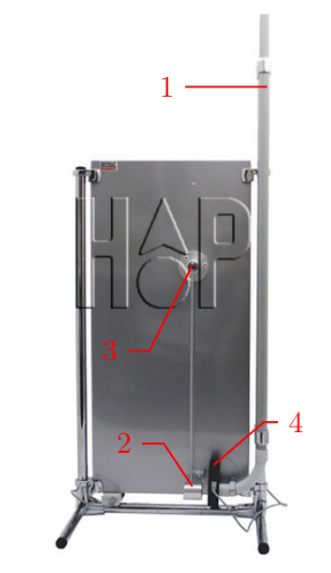
\includegraphics[scale=0.5]{scheme}
	\end{figure}
	Лабораторный стенд включает направляющую трубу 1 для фиксации траектории движения шарика, баллистический маятник с конусом-уловителем 2, датчик угла отклонения маятника 3 на его оси, оптический датчик 4 для определения скорости вылета шарика. К приборам и принадлежностям относятся также компьютер с необходимым программным обеспечением, концентратор для подключения датчика к компьютеру и металлический шарик.
	\section{Порядок действий}
	1)Соберем экспериментальную установку.\\
	2)Запустим измерения на компьютере и отпустим шарик в трубу.\\
	3)После отклонения на максимальный угол остановим измерения.\\
	4)Повторим эксперимент еще 4 раза.
	\section{Таблицы данных и графики}
		\begin{figure}[H]
		\centering
		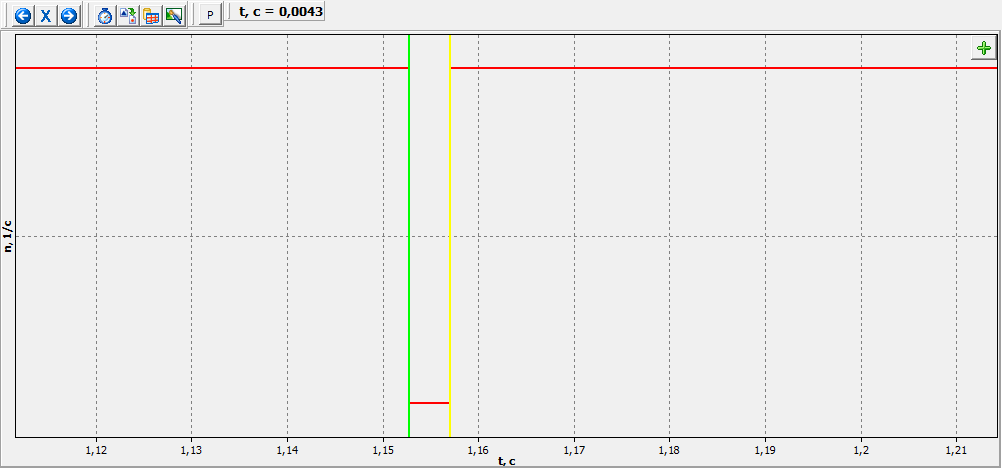
\includegraphics[scale=0.4]{hell1}
		\caption{График перекрытия оптического датчика}
	\end{figure}
	\begin{figure}[H]
		\centering
		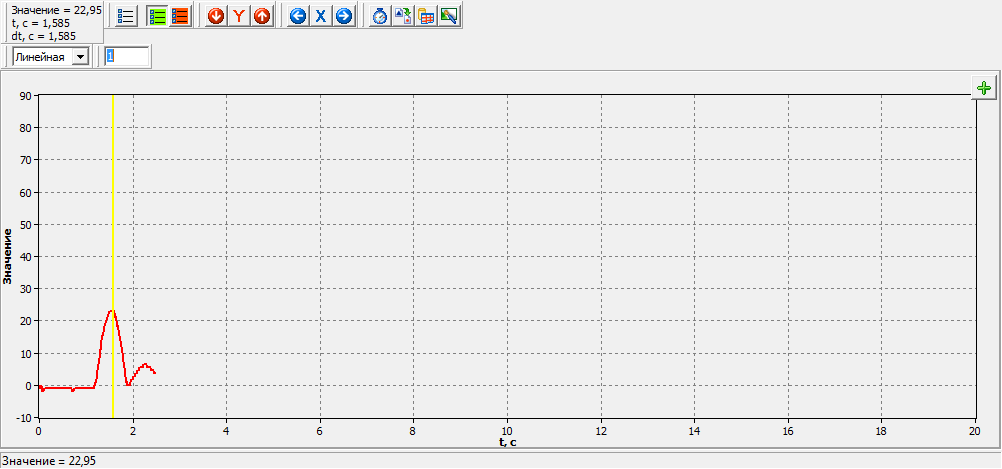
\includegraphics[scale=0.4]{hell2}
		\caption{График зависимости угла отклонения маятника от времени}
	\end{figure}
	\begin{table}[H]
		\begin{tabular}{|l|l|l|l|l|}
			\hline
			$m$, г       & $d$, мм & $M$, г     & $m_{ct}$, г & $l$, мм       \\ \hline
			24$\pm$0,1 & 18,3    & 55$\pm$0,1 & 34$\pm$0,1  & 509,5$\pm$0,5 \\ \hline
		\end{tabular}
		\caption{}
	\end{table}
	\begin{table}[H]
		\begin{tabular}{|l|l|l|l|l|l|l|}
			\hline
			$i$ & $t_{i imp}$, с & $v_{i opt}$, м/с & $\overline{v}_{opt}$, м/с & $\varphi_{i max}$, град & $v_{i bm}$, м/с & $\overline{v}_{bm}$, м/с \\ \hline
			1   & 0,0041         & 4,46             &                           & 22,04               & 3,315              &                          \\ \cline{1-3} \cline{5-6}
			2   & 0,0040         & 4,58             &                           & 22,04               & 3,315              &                          \\ \cline{1-3} \cline{5-6}
			3   & 0,0038         & 4,82             & 4,604                     & 23,87               & 3,586              & 3,482                    \\ \cline{1-3} \cline{5-6}
			4   & 0,0040         & 4,58             &                           & 22,95               & 3,598              &                          \\ \cline{1-3} \cline{5-6}
			5   & 0,0040         & 4,58             &                           & 22,95               & 3,598              &                          \\ \hline
		\end{tabular}
		\caption{Результаты измерений}
	\end{table}
	\section{Расчеты}
	$v_{opt}=\frac{d}{t_{imp}}$\\
	$v_{bm}=\frac{1}{m}\sqrt{(m+M+\frac{m_{st}}{2})(m+M+\frac{m_{st}}{2})2gl(1-cos\varphi_{max})}$\\
	$\overline{v}=\frac{\sum\limits_{i=1}^{5}v_i}{5}$\\
	$\Delta v_{opt}=2\sqrt{\frac{\sum\limits_{i=1}^5(v_i-\overline{v})}{5}}+\overline{v}\cdot\varepsilon_v=2\sqrt{\frac{\sum\limits_{i=1}^5(v_i-\overline{v})}{5}}+\overline{v}\frac{\Delta t}{\overline{t}}=2\cdot0{,}12+4{,}6\cdot\frac{0{,}0001}{0{,}004}=0{,}355$\\
	$\Delta v_{bm}=2\sqrt{\frac{\sum\limits_{i=1}^5(v_i-\overline{v})}{5}}+\overline{v}\cdot\varepsilon_v=2\sqrt{\frac{\sum\limits_{i=1}^5(v_i-\overline{v})}{5}}+\overline{v}(\frac{\Delta m}{m}+\frac{1}{2}(\frac{\Delta m+\Delta M+\Delta m_{st}/2}{m+M+m_{st}/2}+\frac{\Delta m+\Delta M+\Delta m_{st}/3}{m+M+m_{st}/2}+\frac{\Delta l}{l}+\frac{\Delta cos\varphi_{max}}{1-cos\varphi_{max}})=0{,}305$\\
	$\delta v_{opt}=\frac{\Delta v}{v}=\frac{0{,}355}{4,604}=0{,}08$\\
	$\delta v_{bm}=\frac{\Delta v}{v}=\frac{0{,}305}{3{,}482}=0{,}09$\\
	\section{Результаты}
	$v_{opt}=(4{,}604\pm0{,}355)$ м/с, $\delta v_{opt}=8\%$\\	
	$v_{bm}=(3{,482}\pm0{,}305)$ м/с, $\delta v_{bm}=9\%$\\	
	\section{Вывод}
	Полученные значения отличаются, несмотря на то, что в обоих экспериментах относительная погрешность меньше 10\%. Это можно объяснить тем, что оптический датчик сложно установить так, чтобы шарик перекрывал его всем диаметром, а не частью, поэтому более точным методом является баллистический. 
\end{document}